% ==========================================
% 3. THE MAPPING
% ==========================================
\section{The Mapping: Biology $\cong$ Software}

To treat Agentic Systems and Gene Regulatory Networks (GRNs) as isomorphic, we must map them to a common mathematical object. We utilize the category $\Poly$, where objects are polynomial functors representing interfaces, and morphisms represent interaction protocols.

\subsection{Preliminaries: The Category $\Poly$}
In Applied Category Theory, a \textbf{Polynomial Functor} $P$ represents a typed interface for a dynamical system. It is defined as a sum of representable functors:

\begin{equation}
    P(y) = \sum_{o \in O} y^{I_o}
\end{equation}

Here, $O$ is the set of possible \textbf{Positions} (or Outputs) the system can expose. For each position $o \in O$, there is a set $I_o$ of \textbf{Directions} (or Inputs) required to transition the system to a new state.
\begin{itemize}
    \item The coefficient $o$ represents the \textit{value produced} by the system.
    \item The exponent $I_o$ represents the \textit{capacity to receive} information from the environment.
\end{itemize}
This formalism captures the essence of a ``stateful interface'': the system outputs a value $o$ and then waits for a specific type of input $i \in I_o$ before it can proceed.

% --- FIGURE: THE MUSHROOM DIAGRAM (Standard Poly Visual) ---
\begin{figure}[h]
    \centering
    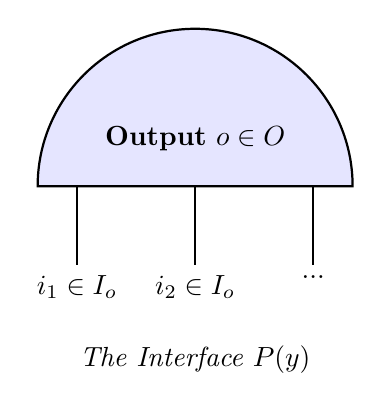
\begin{tikzpicture}
        % The Mushroom Cap (Output/Position)
        \draw[thick, fill=blue!10] (0,1) arc (180:0:2) -- cycle;
        \node at (2, 1.6) {\textbf{Output} $o \in O$};

        % The Stalks (Inputs/Directions)
        \draw[thick] (0.5, 1) -- (0.5, 0) node[below] {$i_1 \in I_o$};
        \draw[thick] (2, 1) -- (2, 0) node[below] {$i_2 \in I_o$};
        \draw[thick] (3.5, 1) -- (3.5, 0) node[below] {$...$};

        % Label
        \node at (2, -1.2) {\textit{The Interface $P(y)$}};
    \end{tikzpicture}
    \caption{A visual representation of a Polynomial Functor (often called a ``Mushroom'' or ``Corolla''). The system offers an Output (the cap) and exposes specific Input ports (the stalks) dependent on that output.}
    \label{fig:poly_mushroom}
\end{figure}

\subsection{The Isomorphism: Genes and Agents}
We now apply this abstract definition to our specific domains.

\begin{definition}[The Gene Object]
A gene $G$ is a polynomial functor where $O_G$ is the set of expressed proteins and $I_G$ is the set of regulatory signals (transcription factors):
\begin{equation}
    P_{Gene}(y) = \sum_{prot \in Proteins} y^{\{TF_{bind}\}}
\end{equation}
\end{definition}

\begin{definition}[The Agent Object]
An autonomous agent $A$ is a polynomial functor where $O_A$ is the set of generated messages, and $I_A$ is the set of observations:
\begin{equation}
    P_{Agent}(y) = \sum_{action \in Actions} y^{\{Obs\}}
\end{equation}
\end{definition}

% ... Continue with "The Interface: Promoters as Lenses" ...

\subsection{The Interface: Promoters as Lenses}

In biology, a gene is not universally accessible. It is guarded by a \textbf{Promoter Region}---a specific DNA sequence that only binds to compatible Transcription Factors. In software, an agent is guarded by an \textbf{API Schema} or Context Window definition.

We model this gating mechanism using \textbf{Optics}, specifically \textbf{Lenses}. A Lens consists of two maps between a global state $S$ and a local view $V$:
\begin{enumerate}
    \item \textbf{Get (View):} $get: S \to V$ (Extracting relevant signal from global state).
    \item \textbf{Put (Update):} $put: S \times V' \to S$ (Updating global state based on local change).
\end{enumerate}

The ``Promoter'' acts as a filter that determines which part of the global cellular environment ($S$) is visible ($V$) to the gene.
\begin{itemize}
    \item \textbf{Biological Lens:} The promoter filters the chaotic cellular soup, allowing the gene to ``see'' only specific molecules (e.g., \textit{Lac Repressor}).
    \item \textbf{Agentic Lens:} The Context Window filters the massive vector database, allowing the agent to ``see'' only the relevant retrieved chunks (RAG).
\end{itemize}

If the input signal does not match the Schema (Promoter), the Lens fails to focus, and the interaction is mathematically undefined (the agent does not run; the gene is not expressed).

\subsection{Epigenetics and State: The Coalgebra}

Neither genes nor agents are stateless functions. They possess memory.
\begin{itemize}
    \item \textbf{Biology:} Epigenetic markers (Methylation, Histone modification) alter how a gene responds to signals without changing the DNA code.
    \item \textbf{Software:} Retrieval Augmented Generation (RAG) and Conversation History alter how an agent responds to a prompt without changing the LLM weights.
\end{itemize}

We model this as a \textbf{Coalgebra} for the polynomial functor $P$. A dynamical system is defined as a tuple $(S, \phi)$, where $S$ is the state space and $\phi$ is the structure map:

\begin{equation}
    \phi: S \to P(S)
\end{equation}

By expanding $P(S)$, we derive the two fundamental operations of the state machine:
\begin{enumerate}
    \item \textbf{Readout:} $S \to O$ (Given current state/memory, what action do I take?)
    \item \textbf{Update:} $S \times I \to S$ (Given current state and new input, what is my new state?)
\end{enumerate}

By establishing this formal dictionary (Table \ref{tab:dictionary}), we assert that GRNs and Agentic Systems are distinct implementations of the same abstract dynamical system.

% --- FIGURE: THE ISOMORPHISM ---
\begin{figure}[h]
    \centering
    \begin{tikzpicture}[
        node distance=2.5cm,
        box/.style={draw, rectangle, rounded corners, minimum width=3cm, minimum height=1.5cm, align=center, thick},
        arrow/.style={->, >=Stealth, very thick}
    ]
        % Left Side: Biology
        \node[box, fill=green!10, draw=green!60!black] (gene) {\textbf{Gene} \\ (Function)};
        \node[above=0.8cm of gene] (tf) {\textit{Transcription Factors} ($I$)};
        \node[below=0.8cm of gene] (prot) {\textit{Proteins} ($O$)};

        \draw[arrow] (tf) -- node[right, font=\footnotesize] {Promoter Binding} (gene);
        \draw[arrow] (gene) -- node[right, font=\footnotesize] {Expression} (prot);

        % Right Side: Software
        \node[box, fill=blue!10, draw=blue!60!black, right=5cm of gene] (agent) {\textbf{Agent} \\ (LLM + Tools)};
        \node[above=0.8cm of agent] (obs) {\textit{Observations} ($I$)};
        \node[below=0.8cm of agent] (act) {\textit{Actions} ($O$)};

        \draw[arrow] (obs) -- node[right, font=\footnotesize] {Schema Match} (agent);
        \draw[arrow] (agent) -- node[right, font=\footnotesize] {Generation} (act);

        % Mapping arrows
        \draw[<->, dashed, ultra thick, color=gray] (gene) -- node[above, font=\bfseries] {Isomorphism $\cong$} (agent);
        \node[below=1.8cm of gene, font=\small, color=gray] {Category $\Poly$};
        \node[below=1.8cm of agent, font=\small, color=gray] {Category $\Poly$};
    \end{tikzpicture}
    \caption{The Structural Isomorphism. Both Genes and Agents act as transducers converting Input Contexts ($I$) into Output Expressions ($O$), governed by the same categorical laws.}
    \label{fig:iso}
\end{figure}

\begin{table}[h]
    \centering
    \renewcommand{\arraystretch}{1.5}
    \begin{tabular}{|l|l|l|}
    \hline
    \textbf{Category Concept} & \textbf{Biological Realization (GRN)} & \textbf{Software Realization (Agentic)} \\ \hline
    Polynomial Functor ($P$) & Gene Interface & Agent Interface (System Prompt) \\ \hline
    Output Position ($O$) & Protein Expression & Tool Call / Message \\ \hline
    Input Direction ($I$) & Transcription Factor Binding & Observation / User Prompt \\ \hline
    Lens (Optic) & Promoter Region & API Schema / Context Window \\ \hline
    Internal State ($S$) & Epigenetic Markers (Methylation) & Vector Store / Chat History \\ \hline
    Morphism ($\circ$) & Signal Transduction Pathway & Data Pipeline \\ \hline
    \end{tabular}
    \caption{The Isomorphism Dictionary}
    \label{tab:dictionary}
\end{table}
